% Created by tikzDevice version 0.12.3 on 2020-09-01 15:22:38
% !TEX encoding = UTF-8 Unicode
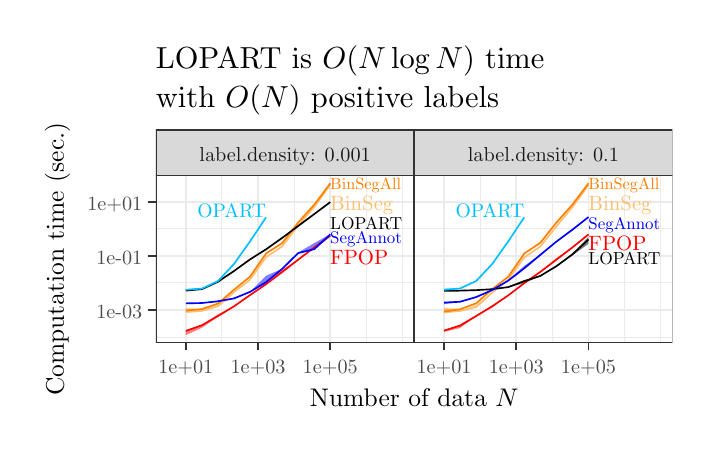
\begin{tikzpicture}[x=1pt,y=1pt]
\definecolor{fillColor}{RGB}{255,255,255}
\path[use as bounding box,fill=fillColor,fill opacity=0.00] (0,0) rectangle (238.49,144.54);
\begin{scope}
\path[clip] (  0.00,  0.00) rectangle (238.49,144.54);
\definecolor{drawColor}{RGB}{255,255,255}
\definecolor{fillColor}{RGB}{255,255,255}

\path[draw=drawColor,line width= 0.6pt,line join=round,line cap=round,fill=fillColor] ( -0.00,  0.00) rectangle (238.49,144.54);
\end{scope}
\begin{scope}
\path[clip] ( 46.36, 30.69) rectangle (139.68, 91.06);
\definecolor{fillColor}{RGB}{255,255,255}

\path[fill=fillColor] ( 46.36, 30.69) rectangle (139.68, 91.06);
\definecolor{drawColor}{gray}{0.92}

\path[draw=drawColor,line width= 0.3pt,line join=round] ( 46.36, 32.77) --
	(139.68, 32.77);

\path[draw=drawColor,line width= 0.3pt,line join=round] ( 46.36, 52.31) --
	(139.68, 52.31);

\path[draw=drawColor,line width= 0.3pt,line join=round] ( 46.36, 71.86) --
	(139.68, 71.86);

\path[draw=drawColor,line width= 0.3pt,line join=round] ( 70.18, 30.69) --
	( 70.18, 91.06);

\path[draw=drawColor,line width= 0.3pt,line join=round] ( 96.28, 30.69) --
	( 96.28, 91.06);

\path[draw=drawColor,line width= 0.3pt,line join=round] (122.39, 30.69) --
	(122.39, 91.06);

\path[draw=drawColor,line width= 0.3pt,line join=round] (135.44, 30.69) --
	(135.44, 91.06);

\path[draw=drawColor,line width= 0.6pt,line join=round] ( 46.36, 42.54) --
	(139.68, 42.54);

\path[draw=drawColor,line width= 0.6pt,line join=round] ( 46.36, 62.09) --
	(139.68, 62.09);

\path[draw=drawColor,line width= 0.6pt,line join=round] ( 46.36, 81.63) --
	(139.68, 81.63);

\path[draw=drawColor,line width= 0.6pt,line join=round] ( 57.13, 30.69) --
	( 57.13, 91.06);

\path[draw=drawColor,line width= 0.6pt,line join=round] ( 83.23, 30.69) --
	( 83.23, 91.06);

\path[draw=drawColor,line width= 0.6pt,line join=round] (109.33, 30.69) --
	(109.33, 91.06);
\definecolor{fillColor}{RGB}{253,191,111}

\path[fill=fillColor,fill opacity=0.50] ( 57.13, 41.93) --
	( 62.97, 42.39) --
	( 68.77, 44.27) --
	( 74.55, 49.03) --
	( 80.34, 53.48) --
	( 86.14, 61.63) --
	( 91.93, 65.50) --
	( 97.73, 73.02) --
	(103.53, 79.73) --
	(109.33, 87.71) --
	(109.33, 87.71) --
	(103.53, 79.72) --
	( 97.73, 73.01) --
	( 91.93, 65.49) --
	( 86.14, 61.62) --
	( 80.34, 53.44) --
	( 74.55, 48.86) --
	( 68.77, 43.64) --
	( 62.97, 41.85) --
	( 57.13, 41.45) --
	cycle;

\path[] ( 57.13, 41.93) --
	( 62.97, 42.39) --
	( 68.77, 44.27) --
	( 74.55, 49.03) --
	( 80.34, 53.48) --
	( 86.14, 61.63) --
	( 91.93, 65.50) --
	( 97.73, 73.02) --
	(103.53, 79.73) --
	(109.33, 87.71);

\path[] (109.33, 87.71) --
	(103.53, 79.72) --
	( 97.73, 73.01) --
	( 91.93, 65.49) --
	( 86.14, 61.62) --
	( 80.34, 53.44) --
	( 74.55, 48.86) --
	( 68.77, 43.64) --
	( 62.97, 41.85) --
	( 57.13, 41.45);
\definecolor{fillColor}{RGB}{255,127,0}

\path[fill=fillColor,fill opacity=0.50] ( 57.13, 43.10) --
	( 62.97, 42.92) --
	( 68.77, 44.92) --
	( 74.55, 49.91) --
	( 80.34, 54.57) --
	( 86.14, 62.96) --
	( 91.93, 66.74) --
	( 97.73, 74.14) --
	(103.53, 80.58) --
	(109.33, 88.29) --
	(109.33, 88.29) --
	(103.53, 80.55) --
	( 97.73, 74.09) --
	( 91.93, 66.64) --
	( 86.14, 62.94) --
	( 80.34, 54.52) --
	( 74.55, 49.85) --
	( 68.77, 44.63) --
	( 62.97, 42.45) --
	( 57.13, 41.98) --
	cycle;

\path[] ( 57.13, 43.10) --
	( 62.97, 42.92) --
	( 68.77, 44.92) --
	( 74.55, 49.91) --
	( 80.34, 54.57) --
	( 86.14, 62.96) --
	( 91.93, 66.74) --
	( 97.73, 74.14) --
	(103.53, 80.58) --
	(109.33, 88.29);

\path[] (109.33, 88.29) --
	(103.53, 80.55) --
	( 97.73, 74.09) --
	( 91.93, 66.64) --
	( 86.14, 62.94) --
	( 80.34, 54.52) --
	( 74.55, 49.85) --
	( 68.77, 44.63) --
	( 62.97, 42.45) --
	( 57.13, 41.98);
\definecolor{fillColor}{RGB}{255,0,0}

\path[fill=fillColor,fill opacity=0.50] ( 57.13, 35.07) --
	( 62.97, 37.26) --
	( 68.77, 40.94) --
	( 74.55, 43.94) --
	( 80.34, 47.92) --
	( 86.14, 51.98) --
	( 91.93, 57.08) --
	( 97.73, 60.87) --
	(103.53, 65.13) --
	(109.33, 69.46) --
	(109.33, 69.34) --
	(103.53, 65.11) --
	( 97.73, 60.54) --
	( 91.93, 56.18) --
	( 86.14, 51.81) --
	( 80.34, 47.77) --
	( 74.55, 43.79) --
	( 68.77, 40.13) --
	( 62.97, 36.08) --
	( 57.13, 33.43) --
	cycle;

\path[] ( 57.13, 35.07) --
	( 62.97, 37.26) --
	( 68.77, 40.94) --
	( 74.55, 43.94) --
	( 80.34, 47.92) --
	( 86.14, 51.98) --
	( 91.93, 57.08) --
	( 97.73, 60.87) --
	(103.53, 65.13) --
	(109.33, 69.46);

\path[] (109.33, 69.34) --
	(103.53, 65.11) --
	( 97.73, 60.54) --
	( 91.93, 56.18) --
	( 86.14, 51.81) --
	( 80.34, 47.77) --
	( 74.55, 43.79) --
	( 68.77, 40.13) --
	( 62.97, 36.08) --
	( 57.13, 33.43);
\definecolor{fillColor}{RGB}{0,0,0}

\path[fill=fillColor,fill opacity=0.50] ( 57.13, 49.98) --
	( 62.97, 50.32) --
	( 68.77, 52.76) --
	( 74.55, 56.63) --
	( 80.34, 60.79) --
	( 86.14, 64.45) --
	( 91.93, 68.56) --
	( 97.73, 72.88) --
	(103.53, 77.17) --
	(109.33, 81.55) --
	(109.33, 81.49) --
	(103.53, 77.16) --
	( 97.73, 72.86) --
	( 91.93, 68.55) --
	( 86.14, 64.44) --
	( 80.34, 60.79) --
	( 74.55, 56.59) --
	( 68.77, 52.67) --
	( 62.97, 50.03) --
	( 57.13, 49.47) --
	cycle;

\path[] ( 57.13, 49.98) --
	( 62.97, 50.32) --
	( 68.77, 52.76) --
	( 74.55, 56.63) --
	( 80.34, 60.79) --
	( 86.14, 64.45) --
	( 91.93, 68.56) --
	( 97.73, 72.88) --
	(103.53, 77.17) --
	(109.33, 81.55);

\path[] (109.33, 81.49) --
	(103.53, 77.16) --
	( 97.73, 72.86) --
	( 91.93, 68.55) --
	( 86.14, 64.44) --
	( 80.34, 60.79) --
	( 74.55, 56.59) --
	( 68.77, 52.67) --
	( 62.97, 50.03) --
	( 57.13, 49.47);
\definecolor{fillColor}{RGB}{0,191,255}

\path[fill=fillColor,fill opacity=0.50] ( 57.13, 49.89) --
	( 62.97, 50.36) --
	( 68.77, 53.00) --
	( 74.55, 59.16) --
	( 80.34, 67.30) --
	( 86.14, 76.01) --
	( 86.14, 75.99) --
	( 80.34, 67.30) --
	( 74.55, 59.13) --
	( 68.77, 52.83) --
	( 62.97, 50.23) --
	( 57.13, 49.77) --
	cycle;

\path[] ( 57.13, 49.89) --
	( 62.97, 50.36) --
	( 68.77, 53.00) --
	( 74.55, 59.16) --
	( 80.34, 67.30) --
	( 86.14, 76.01);

\path[] ( 86.14, 75.99) --
	( 80.34, 67.30) --
	( 74.55, 59.13) --
	( 68.77, 52.83) --
	( 62.97, 50.23) --
	( 57.13, 49.77);
\definecolor{fillColor}{RGB}{0,0,255}

\path[fill=fillColor,fill opacity=0.50] ( 57.13, 44.96) --
	( 62.97, 45.07) --
	( 68.77, 45.83) --
	( 74.55, 46.90) --
	( 80.34, 49.12) --
	( 86.14, 54.90) --
	( 91.93, 57.38) --
	( 97.73, 63.30) --
	(103.53, 66.68) --
	(109.33, 69.87) --
	(109.33, 68.96) --
	(103.53, 64.41) --
	( 97.73, 63.08) --
	( 91.93, 57.35) --
	( 86.14, 52.50) --
	( 80.34, 48.79) --
	( 74.55, 46.68) --
	( 68.77, 45.43) --
	( 62.97, 44.96) --
	( 57.13, 44.91) --
	cycle;

\path[] ( 57.13, 44.96) --
	( 62.97, 45.07) --
	( 68.77, 45.83) --
	( 74.55, 46.90) --
	( 80.34, 49.12) --
	( 86.14, 54.90) --
	( 91.93, 57.38) --
	( 97.73, 63.30) --
	(103.53, 66.68) --
	(109.33, 69.87);

\path[] (109.33, 68.96) --
	(103.53, 64.41) --
	( 97.73, 63.08) --
	( 91.93, 57.35) --
	( 86.14, 52.50) --
	( 80.34, 48.79) --
	( 74.55, 46.68) --
	( 68.77, 45.43) --
	( 62.97, 44.96) --
	( 57.13, 44.91);
\definecolor{drawColor}{RGB}{253,191,111}

\path[draw=drawColor,line width= 0.6pt,line join=round] ( 57.13, 41.83) --
	( 62.97, 42.23) --
	( 68.77, 43.90) --
	( 74.55, 48.96) --
	( 80.34, 53.47) --
	( 86.14, 61.62) --
	( 91.93, 65.49) --
	( 97.73, 73.01) --
	(103.53, 79.73) --
	(109.33, 87.71);
\definecolor{drawColor}{RGB}{255,127,0}

\path[draw=drawColor,line width= 0.6pt,line join=round] ( 57.13, 42.32) --
	( 62.97, 42.86) --
	( 68.77, 44.83) --
	( 74.55, 49.85) --
	( 80.34, 54.56) --
	( 86.14, 62.94) --
	( 91.93, 66.65) --
	( 97.73, 74.11) --
	(103.53, 80.55) --
	(109.33, 88.29);
\definecolor{drawColor}{RGB}{255,0,0}

\path[draw=drawColor,line width= 0.6pt,line join=round] ( 57.13, 34.97) --
	( 62.97, 37.00) --
	( 68.77, 40.35) --
	( 74.55, 43.84) --
	( 80.34, 47.90) --
	( 86.14, 51.84) --
	( 91.93, 56.21) --
	( 97.73, 60.68) --
	(103.53, 65.12) --
	(109.33, 69.37);
\definecolor{drawColor}{RGB}{0,0,0}

\path[draw=drawColor,line width= 0.6pt,line join=round] ( 57.13, 49.52) --
	( 62.97, 50.06) --
	( 68.77, 52.72) --
	( 74.55, 56.61) --
	( 80.34, 60.79) --
	( 86.14, 64.45) --
	( 91.93, 68.55) --
	( 97.73, 72.87) --
	(103.53, 77.17) --
	(109.33, 81.50);
\definecolor{drawColor}{RGB}{0,191,255}

\path[draw=drawColor,line width= 0.6pt,line join=round] ( 57.13, 49.84) --
	( 62.97, 50.25) --
	( 68.77, 52.98) --
	( 74.55, 59.15) --
	( 80.34, 67.30) --
	( 86.14, 76.00);
\definecolor{drawColor}{RGB}{0,0,255}

\path[draw=drawColor,line width= 0.6pt,line join=round] ( 57.13, 44.92) --
	( 62.97, 45.04) --
	( 68.77, 45.68) --
	( 74.55, 46.69) --
	( 80.34, 49.07) --
	( 86.14, 52.57) --
	( 91.93, 57.36) --
	( 97.73, 63.08) --
	(103.53, 64.48) --
	(109.33, 69.86);
\end{scope}
\begin{scope}
\path[clip] ( 46.36, 30.69) rectangle (139.68, 91.06);
\definecolor{drawColor}{RGB}{255,0,0}

\node[text=drawColor,anchor=base west,inner sep=0pt, outer sep=0pt, scale=  0.75] at (109.33, 58.99) {FPOP};
\definecolor{drawColor}{RGB}{0,0,255}

\node[text=drawColor,anchor=base west,inner sep=0pt, outer sep=0pt, scale=  0.61] at (109.33, 66.61) {SegAnnot};
\definecolor{drawColor}{RGB}{0,0,0}

\node[text=drawColor,anchor=base west,inner sep=0pt, outer sep=0pt, scale=  0.63] at (109.33, 71.63) {LOPART};
\definecolor{drawColor}{RGB}{253,191,111}

\node[text=drawColor,anchor=base west,inner sep=0pt, outer sep=0pt, scale=  0.75] at (109.33, 78.56) {BinSeg};
\definecolor{drawColor}{RGB}{255,127,0}

\node[text=drawColor,anchor=base west,inner sep=0pt, outer sep=0pt, scale=  0.59] at (109.33, 86.14) {BinSegAll};
\definecolor{drawColor}{RGB}{0,191,255}

\node[text=drawColor,anchor=base east,inner sep=0pt, outer sep=0pt, scale=  0.71] at ( 86.14, 76.00) {OPART};
\definecolor{drawColor}{gray}{0.20}

\path[draw=drawColor,line width= 0.6pt,line join=round,line cap=round] ( 46.36, 30.69) rectangle (139.68, 91.06);
\end{scope}
\begin{scope}
\path[clip] (139.68, 30.69) rectangle (232.99, 91.06);
\definecolor{fillColor}{RGB}{255,255,255}

\path[fill=fillColor] (139.68, 30.69) rectangle (232.99, 91.06);
\definecolor{drawColor}{gray}{0.92}

\path[draw=drawColor,line width= 0.3pt,line join=round] (139.68, 32.77) --
	(232.99, 32.77);

\path[draw=drawColor,line width= 0.3pt,line join=round] (139.68, 52.31) --
	(232.99, 52.31);

\path[draw=drawColor,line width= 0.3pt,line join=round] (139.68, 71.86) --
	(232.99, 71.86);

\path[draw=drawColor,line width= 0.3pt,line join=round] (163.50, 30.69) --
	(163.50, 91.06);

\path[draw=drawColor,line width= 0.3pt,line join=round] (189.60, 30.69) --
	(189.60, 91.06);

\path[draw=drawColor,line width= 0.3pt,line join=round] (215.70, 30.69) --
	(215.70, 91.06);

\path[draw=drawColor,line width= 0.3pt,line join=round] (228.75, 30.69) --
	(228.75, 91.06);

\path[draw=drawColor,line width= 0.6pt,line join=round] (139.68, 42.54) --
	(232.99, 42.54);

\path[draw=drawColor,line width= 0.6pt,line join=round] (139.68, 62.09) --
	(232.99, 62.09);

\path[draw=drawColor,line width= 0.6pt,line join=round] (139.68, 81.63) --
	(232.99, 81.63);

\path[draw=drawColor,line width= 0.6pt,line join=round] (150.44, 30.69) --
	(150.44, 91.06);

\path[draw=drawColor,line width= 0.6pt,line join=round] (176.55, 30.69) --
	(176.55, 91.06);

\path[draw=drawColor,line width= 0.6pt,line join=round] (202.65, 30.69) --
	(202.65, 91.06);
\definecolor{fillColor}{RGB}{253,191,111}

\path[fill=fillColor,fill opacity=0.50] (150.44, 41.94) --
	(156.28, 42.18) --
	(162.09, 44.55) --
	(167.86, 49.00) --
	(173.65, 53.55) --
	(179.45, 61.72) --
	(185.25, 65.47) --
	(191.05, 72.76) --
	(196.85, 79.88) --
	(202.65, 87.60) --
	(202.65, 87.60) --
	(196.85, 79.71) --
	(191.05, 72.72) --
	(185.25, 65.46) --
	(179.45, 61.51) --
	(173.65, 53.46) --
	(167.86, 48.69) --
	(162.09, 43.51) --
	(156.28, 42.11) --
	(150.44, 41.31) --
	cycle;

\path[] (150.44, 41.94) --
	(156.28, 42.18) --
	(162.09, 44.55) --
	(167.86, 49.00) --
	(173.65, 53.55) --
	(179.45, 61.72) --
	(185.25, 65.47) --
	(191.05, 72.76) --
	(196.85, 79.88) --
	(202.65, 87.60);

\path[] (202.65, 87.60) --
	(196.85, 79.71) --
	(191.05, 72.72) --
	(185.25, 65.46) --
	(179.45, 61.51) --
	(173.65, 53.46) --
	(167.86, 48.69) --
	(162.09, 43.51) --
	(156.28, 42.11) --
	(150.44, 41.31);
\definecolor{fillColor}{RGB}{255,127,0}

\path[fill=fillColor,fill opacity=0.50] (150.44, 43.19) --
	(156.28, 42.95) --
	(162.09, 45.04) --
	(167.86, 50.14) --
	(173.65, 54.54) --
	(179.45, 63.14) --
	(185.25, 67.12) --
	(191.05, 74.16) --
	(196.85, 80.63) --
	(202.65, 88.31) --
	(202.65, 88.30) --
	(196.85, 80.56) --
	(191.05, 74.12) --
	(185.25, 66.73) --
	(179.45, 62.93) --
	(173.65, 54.51) --
	(167.86, 49.82) --
	(162.09, 44.78) --
	(156.28, 42.61) --
	(150.44, 41.62) --
	cycle;

\path[] (150.44, 43.19) --
	(156.28, 42.95) --
	(162.09, 45.04) --
	(167.86, 50.14) --
	(173.65, 54.54) --
	(179.45, 63.14) --
	(185.25, 67.12) --
	(191.05, 74.16) --
	(196.85, 80.63) --
	(202.65, 88.31);

\path[] (202.65, 88.30) --
	(196.85, 80.56) --
	(191.05, 74.12) --
	(185.25, 66.73) --
	(179.45, 62.93) --
	(173.65, 54.51) --
	(167.86, 49.82) --
	(162.09, 44.78) --
	(156.28, 42.61) --
	(150.44, 41.62);
\definecolor{fillColor}{RGB}{255,0,0}

\path[fill=fillColor,fill opacity=0.50] (150.44, 35.21) --
	(156.28, 37.27) --
	(162.09, 40.73) --
	(167.86, 43.91) --
	(173.65, 47.86) --
	(179.45, 52.37) --
	(185.25, 56.33) --
	(191.05, 61.30) --
	(196.85, 65.17) --
	(202.65, 70.23) --
	(202.65, 69.71) --
	(196.85, 65.00) --
	(191.05, 60.58) --
	(185.25, 56.21) --
	(179.45, 51.99) --
	(173.65, 47.78) --
	(167.86, 43.36) --
	(162.09, 40.32) --
	(156.28, 36.00) --
	(150.44, 34.63) --
	cycle;

\path[] (150.44, 35.21) --
	(156.28, 37.27) --
	(162.09, 40.73) --
	(167.86, 43.91) --
	(173.65, 47.86) --
	(179.45, 52.37) --
	(185.25, 56.33) --
	(191.05, 61.30) --
	(196.85, 65.17) --
	(202.65, 70.23);

\path[] (202.65, 69.71) --
	(196.85, 65.00) --
	(191.05, 60.58) --
	(185.25, 56.21) --
	(179.45, 51.99) --
	(173.65, 47.78) --
	(167.86, 43.36) --
	(162.09, 40.32) --
	(156.28, 36.00) --
	(150.44, 34.63);
\definecolor{fillColor}{RGB}{0,0,0}

\path[fill=fillColor,fill opacity=0.50] (150.44, 49.57) --
	(156.28, 49.77) --
	(162.09, 49.73) --
	(167.86, 50.04) --
	(173.65, 50.92) --
	(179.45, 53.40) --
	(185.25, 54.86) --
	(191.05, 58.35) --
	(196.85, 62.91) --
	(202.65, 68.98) --
	(202.65, 66.41) --
	(196.85, 62.25) --
	(191.05, 58.29) --
	(185.25, 54.82) --
	(179.45, 52.21) --
	(173.65, 50.67) --
	(167.86, 49.94) --
	(162.09, 49.69) --
	(156.28, 49.44) --
	(150.44, 49.40) --
	cycle;

\path[] (150.44, 49.57) --
	(156.28, 49.77) --
	(162.09, 49.73) --
	(167.86, 50.04) --
	(173.65, 50.92) --
	(179.45, 53.40) --
	(185.25, 54.86) --
	(191.05, 58.35) --
	(196.85, 62.91) --
	(202.65, 68.98);

\path[] (202.65, 66.41) --
	(196.85, 62.25) --
	(191.05, 58.29) --
	(185.25, 54.82) --
	(179.45, 52.21) --
	(173.65, 50.67) --
	(167.86, 49.94) --
	(162.09, 49.69) --
	(156.28, 49.44) --
	(150.44, 49.40);
\definecolor{fillColor}{RGB}{0,191,255}

\path[fill=fillColor,fill opacity=0.50] (150.44, 50.28) --
	(156.28, 50.40) --
	(162.09, 53.18) --
	(167.86, 59.18) --
	(173.65, 67.31) --
	(179.45, 76.10) --
	(179.45, 76.00) --
	(173.65, 67.30) --
	(167.86, 59.13) --
	(162.09, 52.99) --
	(156.28, 50.25) --
	(150.44, 49.81) --
	cycle;

\path[] (150.44, 50.28) --
	(156.28, 50.40) --
	(162.09, 53.18) --
	(167.86, 59.18) --
	(173.65, 67.31) --
	(179.45, 76.10);

\path[] (179.45, 76.00) --
	(173.65, 67.30) --
	(167.86, 59.13) --
	(162.09, 52.99) --
	(156.28, 50.25) --
	(150.44, 49.81);
\definecolor{fillColor}{RGB}{0,0,255}

\path[fill=fillColor,fill opacity=0.50] (150.44, 45.33) --
	(156.28, 45.77) --
	(162.09, 47.24) --
	(167.86, 49.74) --
	(173.65, 53.31) --
	(179.45, 58.49) --
	(185.25, 62.51) --
	(191.05, 67.25) --
	(196.85, 71.61) --
	(202.65, 76.24) --
	(202.65, 76.01) --
	(196.85, 71.21) --
	(191.05, 67.22) --
	(185.25, 62.05) --
	(179.45, 57.49) --
	(173.65, 53.12) --
	(167.86, 49.70) --
	(162.09, 47.02) --
	(156.28, 45.40) --
	(150.44, 44.62) --
	cycle;

\path[] (150.44, 45.33) --
	(156.28, 45.77) --
	(162.09, 47.24) --
	(167.86, 49.74) --
	(173.65, 53.31) --
	(179.45, 58.49) --
	(185.25, 62.51) --
	(191.05, 67.25) --
	(196.85, 71.61) --
	(202.65, 76.24);

\path[] (202.65, 76.01) --
	(196.85, 71.21) --
	(191.05, 67.22) --
	(185.25, 62.05) --
	(179.45, 57.49) --
	(173.65, 53.12) --
	(167.86, 49.70) --
	(162.09, 47.02) --
	(156.28, 45.40) --
	(150.44, 44.62);
\definecolor{drawColor}{RGB}{253,191,111}

\path[draw=drawColor,line width= 0.6pt,line join=round] (150.44, 41.69) --
	(156.28, 42.17) --
	(162.09, 43.62) --
	(167.86, 48.84) --
	(173.65, 53.46) --
	(179.45, 61.52) --
	(185.25, 65.47) --
	(191.05, 72.73) --
	(196.85, 79.72) --
	(202.65, 87.60);
\definecolor{drawColor}{RGB}{255,127,0}

\path[draw=drawColor,line width= 0.6pt,line join=round] (150.44, 41.95) --
	(156.28, 42.78) --
	(162.09, 44.95) --
	(167.86, 50.08) --
	(173.65, 54.53) --
	(179.45, 62.93) --
	(185.25, 66.79) --
	(191.05, 74.13) --
	(196.85, 80.61) --
	(202.65, 88.31);
\definecolor{drawColor}{RGB}{255,0,0}

\path[draw=drawColor,line width= 0.6pt,line join=round] (150.44, 35.06) --
	(156.28, 36.91) --
	(162.09, 40.33) --
	(167.86, 43.88) --
	(173.65, 47.80) --
	(179.45, 52.23) --
	(185.25, 56.30) --
	(191.05, 60.70) --
	(196.85, 65.14) --
	(202.65, 69.82);
\definecolor{drawColor}{RGB}{0,0,0}

\path[draw=drawColor,line width= 0.6pt,line join=round] (150.44, 49.43) --
	(156.28, 49.51) --
	(162.09, 49.70) --
	(167.86, 50.04) --
	(173.65, 50.80) --
	(179.45, 52.92) --
	(185.25, 54.85) --
	(191.05, 58.34) --
	(196.85, 62.63) --
	(202.65, 67.99);
\definecolor{drawColor}{RGB}{0,191,255}

\path[draw=drawColor,line width= 0.6pt,line join=round] (150.44, 49.81) --
	(156.28, 50.30) --
	(162.09, 53.02) --
	(167.86, 59.15) --
	(173.65, 67.31) --
	(179.45, 76.02);
\definecolor{drawColor}{RGB}{0,0,255}

\path[draw=drawColor,line width= 0.6pt,line join=round] (150.44, 45.20) --
	(156.28, 45.50) --
	(162.09, 47.21) --
	(167.86, 49.73) --
	(173.65, 53.13) --
	(179.45, 57.59) --
	(185.25, 62.46) --
	(191.05, 67.23) --
	(196.85, 71.56) --
	(202.65, 76.10);
\end{scope}
\begin{scope}
\path[clip] (139.68, 30.69) rectangle (232.99, 91.06);
\definecolor{drawColor}{RGB}{0,0,0}

\node[text=drawColor,anchor=base west,inner sep=0pt, outer sep=0pt, scale=  0.63] at (202.65, 58.99) {LOPART};
\definecolor{drawColor}{RGB}{255,0,0}

\node[text=drawColor,anchor=base west,inner sep=0pt, outer sep=0pt, scale=  0.75] at (202.65, 64.17) {FPOP};
\definecolor{drawColor}{RGB}{0,0,255}

\node[text=drawColor,anchor=base west,inner sep=0pt, outer sep=0pt, scale=  0.61] at (202.65, 71.79) {SegAnnot};
\definecolor{drawColor}{RGB}{253,191,111}

\node[text=drawColor,anchor=base west,inner sep=0pt, outer sep=0pt, scale=  0.75] at (202.65, 78.56) {BinSeg};
\definecolor{drawColor}{RGB}{255,127,0}

\node[text=drawColor,anchor=base west,inner sep=0pt, outer sep=0pt, scale=  0.59] at (202.65, 86.14) {BinSegAll};
\definecolor{drawColor}{RGB}{0,191,255}

\node[text=drawColor,anchor=base east,inner sep=0pt, outer sep=0pt, scale=  0.71] at (179.45, 76.02) {OPART};
\definecolor{drawColor}{gray}{0.20}

\path[draw=drawColor,line width= 0.6pt,line join=round,line cap=round] (139.68, 30.69) rectangle (232.99, 91.06);
\end{scope}
\begin{scope}
\path[clip] ( 46.36, 91.06) rectangle (139.68,107.63);
\definecolor{drawColor}{gray}{0.20}
\definecolor{fillColor}{gray}{0.85}

\path[draw=drawColor,line width= 0.6pt,line join=round,line cap=round,fill=fillColor] ( 46.36, 91.06) rectangle (139.68,107.63);
\definecolor{drawColor}{gray}{0.10}

\node[text=drawColor,anchor=base,inner sep=0pt, outer sep=0pt, scale=  0.73] at ( 93.02, 96.31) {label.density: 0.001};
\end{scope}
\begin{scope}
\path[clip] (139.68, 91.06) rectangle (232.99,107.63);
\definecolor{drawColor}{gray}{0.20}
\definecolor{fillColor}{gray}{0.85}

\path[draw=drawColor,line width= 0.6pt,line join=round,line cap=round,fill=fillColor] (139.68, 91.06) rectangle (232.99,107.63);
\definecolor{drawColor}{gray}{0.10}

\node[text=drawColor,anchor=base,inner sep=0pt, outer sep=0pt, scale=  0.73] at (186.33, 96.31) {label.density: 0.1};
\end{scope}
\begin{scope}
\path[clip] (  0.00,  0.00) rectangle (238.49,144.54);
\definecolor{drawColor}{gray}{0.20}

\path[draw=drawColor,line width= 0.6pt,line join=round] ( 57.13, 27.94) --
	( 57.13, 30.69);

\path[draw=drawColor,line width= 0.6pt,line join=round] ( 83.23, 27.94) --
	( 83.23, 30.69);

\path[draw=drawColor,line width= 0.6pt,line join=round] (109.33, 27.94) --
	(109.33, 30.69);
\end{scope}
\begin{scope}
\path[clip] (  0.00,  0.00) rectangle (238.49,144.54);
\definecolor{drawColor}{gray}{0.30}

\node[text=drawColor,anchor=base,inner sep=0pt, outer sep=0pt, scale=  0.73] at ( 57.13, 19.68) {1e+01};

\node[text=drawColor,anchor=base,inner sep=0pt, outer sep=0pt, scale=  0.73] at ( 83.23, 19.68) {1e+03};

\node[text=drawColor,anchor=base,inner sep=0pt, outer sep=0pt, scale=  0.73] at (109.33, 19.68) {1e+05};
\end{scope}
\begin{scope}
\path[clip] (  0.00,  0.00) rectangle (238.49,144.54);
\definecolor{drawColor}{gray}{0.20}

\path[draw=drawColor,line width= 0.6pt,line join=round] (150.44, 27.94) --
	(150.44, 30.69);

\path[draw=drawColor,line width= 0.6pt,line join=round] (176.55, 27.94) --
	(176.55, 30.69);

\path[draw=drawColor,line width= 0.6pt,line join=round] (202.65, 27.94) --
	(202.65, 30.69);
\end{scope}
\begin{scope}
\path[clip] (  0.00,  0.00) rectangle (238.49,144.54);
\definecolor{drawColor}{gray}{0.30}

\node[text=drawColor,anchor=base,inner sep=0pt, outer sep=0pt, scale=  0.73] at (150.44, 19.68) {1e+01};

\node[text=drawColor,anchor=base,inner sep=0pt, outer sep=0pt, scale=  0.73] at (176.55, 19.68) {1e+03};

\node[text=drawColor,anchor=base,inner sep=0pt, outer sep=0pt, scale=  0.73] at (202.65, 19.68) {1e+05};
\end{scope}
\begin{scope}
\path[clip] (  0.00,  0.00) rectangle (238.49,144.54);
\definecolor{drawColor}{gray}{0.30}

\node[text=drawColor,anchor=base east,inner sep=0pt, outer sep=0pt, scale=  0.73] at ( 41.41, 39.51) {1e-03};

\node[text=drawColor,anchor=base east,inner sep=0pt, outer sep=0pt, scale=  0.73] at ( 41.41, 59.06) {1e-01};

\node[text=drawColor,anchor=base east,inner sep=0pt, outer sep=0pt, scale=  0.73] at ( 41.41, 78.60) {1e+01};
\end{scope}
\begin{scope}
\path[clip] (  0.00,  0.00) rectangle (238.49,144.54);
\definecolor{drawColor}{gray}{0.20}

\path[draw=drawColor,line width= 0.6pt,line join=round] ( 43.61, 42.54) --
	( 46.36, 42.54);

\path[draw=drawColor,line width= 0.6pt,line join=round] ( 43.61, 62.09) --
	( 46.36, 62.09);

\path[draw=drawColor,line width= 0.6pt,line join=round] ( 43.61, 81.63) --
	( 46.36, 81.63);
\end{scope}
\begin{scope}
\path[clip] (  0.00,  0.00) rectangle (238.49,144.54);
\definecolor{drawColor}{RGB}{0,0,0}

\node[text=drawColor,anchor=base,inner sep=0pt, outer sep=0pt, scale=  0.92] at (139.68,  7.64) {Number of data $N$};
\end{scope}
\begin{scope}
\path[clip] (  0.00,  0.00) rectangle (238.49,144.54);
\definecolor{drawColor}{RGB}{0,0,0}

\node[text=drawColor,rotate= 90.00,anchor=base,inner sep=0pt, outer sep=0pt, scale=  0.92] at ( 13.08, 60.87) {Computation time (sec.)};
\end{scope}
\begin{scope}
\path[clip] (  0.00,  0.00) rectangle (238.49,144.54);
\definecolor{drawColor}{RGB}{0,0,0}

\node[text=drawColor,anchor=base west,inner sep=0pt, outer sep=0pt, scale=  1.10] at ( 46.36,129.95) {LOPART is $O(N\log N)$ time};

\node[text=drawColor,anchor=base west,inner sep=0pt, outer sep=0pt, scale=  1.10] at ( 46.36,115.69) {with $O(N)$ positive labels};
\end{scope}
\end{tikzpicture}
